%
% PKUMpLtX --- A LaTeX document class for 'Modern Physics Laboratory' in PKU based on `revtex4-2`
%
% Please read `README.md' and the template file before using
% 需要确保 font 选项指定的字体已安装! 具体参见 `README.md' 的说明.
\documentclass[font=default]{mpltx}

% 以下至 \begin{document} 都仅是本文件为了方便额外定义的命令, 写报告时不需要.
\hypersetup{colorlinks=true}% 超链接带颜色
\usepackage{xcolor}
\newcommand{\note}[1]{{\color{gray}#1}}
\NewDocumentCommand{\pkg}{s o m}{%
    \IfBooleanF{#1}{%
        \IfNoValueTF{#2}%
            {\href{https://www.ctan.org/pkg/#3}}%
            {\href{https://www.ctan.org/pkg/#2}}%
    }%
    {\textsf{#3}}%
}
\newcommand*\cs[1]{\texttt{\textbackslash #1}}
\newcommand*\env[1]{\textit{\texttt{#1}}}
\newcommand*\code[1]{\texttt{#1}}
\newcommand*\file[1]{\textbf{\texttt{#1}}}
\makeatletter
\newcommand\releasedate{%
    \href{https://github.com/CastleStar14654/PKUMpLtX/releases/tag/\mpltx@fileversion}%
        {\mpltx@filedate, \mpltx@fileversion}}
\makeatother
% 以上是本文件为了方便额外定义的命令, 写报告时不需要.

\begin{document}

\title{非线性热对流斑图} % 切合报告内容, 简短明确, 可以不同于讲义
\author{郑熔} % 这里 \emailphone 一定要紧跟在 \author 后方
\emailphone{2300011359@stu.pku.edu.cn}{(86)19805861588}
% 如果改用 \email 则仅需要邮箱参数
\affiliation{北京大学物理学院\quad 学号: 2300011359}
% % 可以使用 \zhdate 自动生成中文日期, 如
\date{\zhdate{2025/9/24}}
% % 也可使用 babel 的 \localedate, 如
% \date{\localedate{2020}{12}{1}}
% % 两者均会输出 `2020 年 12 月 1 日'
% 下面的 \date 的参数是为了自动输出正确版本号, 正式报告请替换为上面的两种 \date 之一
% \date{\releasedate}
\begin{abstract}
  普利高津曾提出关于远离平衡态系统的耗散结构理论: 当开放系统远离平衡态达到一定阈值时, 系统将会出现分岔行为. 在越过分岔点后, 系统将离开原本无序的热力学分支, 突变到一个全新的稳定有序的状态,
  该状态被称为耗散结构.
  瑞利贝纳德对流实验是耗散结构典型实验之一.
  本实验用阴影法观察厚度分别为2 mm 和4 mm 的水层的热对流斑图. 通过改变水层的温度差, 可以观察到斑图随温度差变化的形状变化, 并且记录得到临界点的温度差. 对于2 mm 的水层, 
  临界温度差大约是5.5 \circ C, 对于4 mm 的水层, 临界温度差大约是2.8 \circ C. 通过对实验现象的分析, 可以加深对耗散结构、非线性对流斑图等概念的理解.
 
  % \note{本文档为对 \href{https://github.com/CastleStar14654/PKUMpLtX}{\pkg*{PKUMpLtX}} 的使用示例, 灰色部分为额外针对 \LaTeX{} 模板使用的说明或是一些能提升输出效果的琐碎细节.
    % 也请注意查看源文档 \file{template.tex} 中的注释.}
\end{abstract}
\keywords{耗散结构理论, 非线性对流斑图, 阴影法}

\maketitle

\section{引言}

  1900年, 贝纳对具有自由面-固壁地层的流体薄层进行热对流实验, 观测到了各种对流图形, 现在把底层加热的流体薄层问题统称为贝纳问题. 后来, 瑞利对该问题作了更进一步研究, 故该系统又被称为瑞利贝纳德热对流系统.
  \par
  20世纪六十年代, 普利高津提出耗散结构理论, 指出当一个开放系统原理平衡态达到一定阈值, 系统将会出现分岔行为, 在越过分支后, 系统将会突变进入一个全新的稳定状态. 
  如果将系统拉到离平衡态更远的地方, 系统可能出现更多新的稳定状态. 
  而这种稳定结构被称为耗散结构.
  \par
  以瑞利贝纳德问题为例\autoref{ruilibeinadeduiliu}, 若从动力学角度出发, 通过解 Navier-Stokes 方程, 流体连续性方程, 热传导方程, 并且固定边条件, 可以解得方程组的定常解. 为了了解该定态解的稳定性, 使用线性稳定性分析, 经过一系列计算,
  可以得出临界参量
  $R_c = 1707.76, q_c = 3.117$.
  且边条件$Ra\equiv\frac{g\alpha d^3\delta T}{\nu\kappa}$.
  也就是说当对流水层上下温差使得瑞利数$Ra < R_c$时, 系统出现的扰动会随时间消亡, 定态解会保持稳定; 而反之, 则扰动噪声会逐渐变大, 利用多尺度分析并考虑系统对称性, 可以理解实验中的斑图分岔行为.
  若从热力学角度出发, 由于温度梯度的存在, 且系统为开放系统, 则必有热量的流入和流出. 随着热量的流入和流出, 系统的熵会不断变化. 当熵增小于熵减时, 系统会逐渐变为一个有序结构.
  当维持其有序结构时, 系统会在产生最小熵和最大耗散之间达到一种动态平衡 \cite{jindaiwulishiyan}.
  \par
  阴影法是利用光在不同密度介质中折射率不同来反映液体密度的一种方法. 冷水密度大, 折射率高, 光线穿过其中时汇聚, 在拍摄的照片上会形成亮斑; 热水密度小, 折射率低, 光线穿过其中时发散, 在拍摄的照片上会形成暗斑.
  \par
  本实验利用了一套简易的瑞利贝纳德对流实验系统, 对一小薄层对流水层的下表面进行加热, 在圆形边条件下, 利用阴影法分别观察水层厚度2 mm 和4 mm 的热对流斑图随上下表面温差变化而如何变化,
  并研究瑞利贝纳德对流各个阶段的不同特征, 加深对耗散结构等理论的理解.
  
  \begin{figure}[htbp]
    \centering
    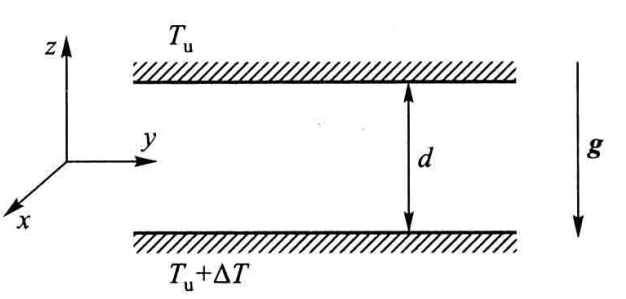
\includegraphics[width=0.85\linewidth]{fig/ruilibeinadeduiliu.png}
    \caption{上下温度不同的两无限大平板间的热对流系统
      }

    \label{fig:ruilibeinadeduiliu}
  \end{figure}


\section{实验}
\subsection{实验装置示意}

\begin{figure}[htbp]
  \centering
  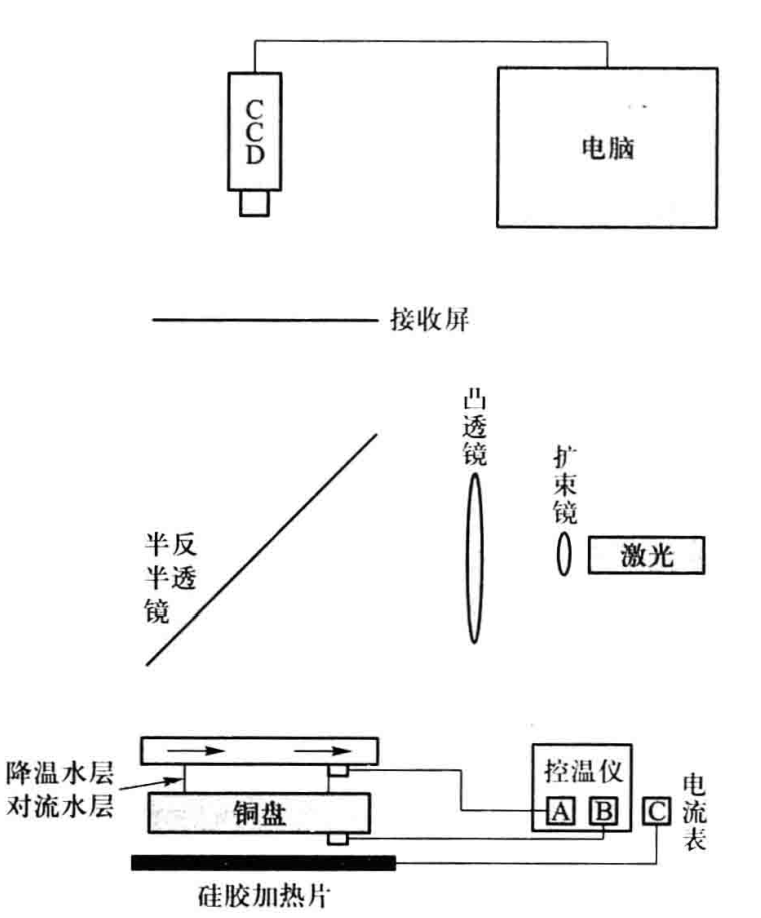
\includegraphics[width=0.85\linewidth]{fig/ruilizhaungzhi.png}
  \caption{非线性对流斑图实验装置示意图
    }
  \label{fig:ruilizhaungzhi}
\end{figure}

  本实验装置如\autoref{fig:ruilizhaungzhi}所示. 研究对象是一薄对流水层. 对流水层上表面有一降温水层, 通过泵入冷水来降低对流水层上表面的温度, 二者的接触面是一蓝宝石片; 
  下表面是一加热铜板, 对其下方的硅胶加热片通电以对对流水层下表面进行加热. 上表面和下表面分别用 Pt100 铂电阻温度计进行测温, 分别通过 A 和 B 温控仪显示. 
  本实验用阴影法观察热对流斑图. 激光发出的光通过扩束器扩束, 经过凸透镜后成为平行光打到半反半透镜上, 经过反射打到降温水层和对流水层, 在水层内部通过折射和反射后,
  重新通过半反半透镜打到接收屏上, 被CCD捕捉.光在不同密度介质中折射率不同. 冷水密度大, 折射率高, 光线穿过其中时汇聚, 在拍摄的照片上会形成亮斑; 热水密度小, 折射率低, 光线穿过其中时发散, 在拍摄的照片上会形成暗斑.
  \par
\subsection{实验步骤}
  \begin{enumerate}
    \item 对流水层的制备. 将厚度为 2 mm 的黑色O环放在铜片上方, 将去离子水加到O环内, 盖上降温水层, 使得对流水层内部无气泡.
    \item 打开激光器, 调整激光器、 扩束器和透镜的位置, 使得光线能够均匀地打到水层和接收屏上.
    \item 开启温控仪电源, 温控仪 A 和 B 分别测量上下表面温度.
    \item 打开水泵, 使冷水流经降温水层.
    \item 逐渐增大硅胶片加热电流, 对流水层上下表面温度差改变, 观察对流水层内热对流斑图的变化并记录相应时刻的温度差.
    \item 将对流水层厚度改为4 mm, 重复步骤1-5.
  \end{enumerate}

\section{结果及讨论}


  \subsection{2 mm 水层的热对流斑图}
  \begin{figure}[htbp]      
    \caption{2 mm 水层的热对流斑图}
    \begin{minipage}{0.32\linewidth}
      \vspace{3pt}
      \centerline{\includegraphics[width=\textwidth]{fig/2mm 0.7A.png}}
      \centerline{I = 0.2 A, $\Delta T = 4.2^\circ C$}
      \vspace{3pt}
      \centerline{\includegraphics[width=\textwidth]{fig/2mm 1A.png}}
      \centerline{I = 1.0 A, $\Delta T = 6.7^\circ C$}
    \end{minipage}
    \begin{minipage}{0.32\linewidth}
      \vspace{3pt}
      \centerline{\includegraphics[width=\textwidth]{fig/2mm 0.8A.png}}
      \centerline{I = 0.8 A, $\Delta T = 5.5^\circ C$}
      \vspace{3pt}
      \centerline{\includegraphics[width=\textwidth]{fig/2mm 1.2A.png}}
      \centerline{I = 1.2 A, $\Delta T = 8.3^\circ C$}
    \end{minipage}
    \label{fig:2mm}
  \end{figure}
  不同电流下的热对流斑图如\autoref{fig:2mm}所示.
  在电流为 0 A 时, 水层上层温度为28.0 \circ C, 下层温度为29.0 \circ C, 这可能是温控仪的接触电阻差异所导致的. 此时图像亮度均匀, 没有出现斑图.
  逐渐增加电流, 水层下表面的温度逐渐增大, 与此同时水层上表面的温度也会增加, 但上表面的增幅小于下表面的增幅. 因此上下表面的温差会逐渐增大.
  \par
  随着电流的增大, 当电流为 0.8 A 时, 上下表面温差达到 5.5 \circ C, 此时可以观察到水层内出现了热对流斑图, 斑图为同心圆状, 系统内部变为有序结构. 该温差即为临界温差.
  电流继续增大, 斑图越来越清晰, 亮线变细, 暗条纹变粗. 这是因为随着温度差的增大, 热上升的水流变多, 而暗条纹对应的是热水. 
  且在温度差达到一定程度时, 斑图结构会发生明显变化, 同心圆结构被破坏, 同心圆的最外围出现鳞片状条纹. 

  \subsection{4 mm 水层的热对流斑图}
  \begin{figure}[htbp]      
    \caption{4 mm 水层的热对流斑图}
    \begin{minipage}{0.32\linewidth}
      \vspace{3pt}
      \centerline{\includegraphics[width=\textwidth]{fig/4mm 0.2A.png}}
      \centerline{I = 0.2 A, $\Delta T = 0.8^\circ C$}
      \vspace{3pt}
      \centerline{\includegraphics[width=\textwidth]{fig/4mm 1.2A.png}}
      \centerline{I = 1.2 A, $\Delta T = 7.7^\circ C$}
    \end{minipage}
    \begin{minipage}{0.32\linewidth}
      \vspace{3pt}
      \centerline{\includegraphics[width=\textwidth]{fig/4mm 0.6A.png}}
      \centerline{I = 0.6 A, $\Delta T = 2.8^\circ C$}
      \vspace{3pt}
      \centerline{\includegraphics[width=\textwidth]{fig/4mm 1.5A.png}}
      \centerline{I = 1.5 A, $\Delta T = 11.1^\circ C$}
    \end{minipage}
    \begin{minipage}{0.32\linewidth}
      \vspace{3pt}
      \centerline{\includegraphics[width=\textwidth]{fig/4mm 0.9A.png}}
      \centerline{I = 0.9 A, $\Delta T = 4.8^\circ C$}
      \vspace{3pt}
      \centerline{\includegraphics[width=\textwidth]{fig/4mm 1.8A.png}}
      \centerline{I = 1.8 A, $\Delta T = 14.3^\circ C$}
    \end{minipage}
    \label{fig:4mm}
  \end{figure}
  不同电流下的热对流斑图如\autoref{fig:4mm}所示.
  在电流为 0 A 时, 水层上层温度为31.4 \circ C, 下层温度为32.2 \circ C, 这可能是温控仪的接触电阻差异所导致的. 此时图像亮度均匀, 没有出现斑图.
  随着电流的增大, 当电流为 0.6 A 时, 上下表面温差达到 2.8 \circ C, 此时可以观察到水层内出现了热对流斑图, 斑图为较模糊的同心圆状, 该温差即为临界温差.
  电流继续增大, 亮线和暗线变清晰.
  且在电流增大的过程中, 可以明显看到条纹的不断被吞的过程. 如\autoref{fig:4mm_0.9_1}所示, 该图为电流为 0.9 A 时, 还未达到稳定状态时的斑图, 
  可以图中央有一亮色条纹正在被吞掉. 这是由于圆形边条件下, 边缘的动力学过程较为确定, 而随着温度差的增大, 对流逐渐增强, 对流原包逐渐向圆形扩张, 原胞的数量逐渐减少,
  从而呈现中心条纹被吞的现象.

  \begin{figure}[htbp]
    \centering
    \includegraphics[width=0.85\linewidth]{fig/4mm 0.9_1.png}
    \caption{电流为 0.9 A 时, 还未达到稳定状态时的斑图}
    \label{fig:4mm_0.9_1}
  \end{figure}

  \par
  当电流达到 1.2 A 时, 温差达到 7.7^\circ C, 斑图的规则性被打破, 同心圆形状发生畸变. 呈现出一些分岔结构. 
  当电流达到 1.5 A 时, 温差达到 11.1^\circ C, 斑图呈现出类似分形的结构. 这是因为分形的结构有助于提升系统的对流效率, 使得系统能够更好地将热量从下表面传递到上表面, 从而提升系统的稳定性.
  当电流达到 1.8 A 时, 温差达到 14.3^\circ C, 斑图变得更加复杂, 几乎丧失了稳定结构特征, 此时水层内部呈现复杂的湍流.

  \par
  根据理论计算, $Ra\equiv\frac{g\alpha d^3\delta T}{\nu\kappa}$, 可知$\Delta T \propto \frac{1}{d^3}$, 因此当水层厚度增大一倍时, 临界温差应成为原来的1/8.
  但在本实验中, 2 mm 水层的临界温差为 5.5 \circ C, 4 mm 水层的临界温差为 2.8 \circ C, 相差约为1/2. 可能的原因如下:
  \begin{itemize}
    \item 实验中水层侧壁外界有热交换, 而理论公式的前提假设是无限大的平板.
    \item 实验中CCD的分辨率有限, 恰好出现热对流斑图的时刻通常无法被准确捕捉
    \item 温控仪的测量精度有限, 测量同时受到接触电阻的影响.
  \end{itemize}


\section{结论}
  本实验利用阴影法观察了厚度分别为2 mm 和4 mm 的水层的热对流斑图. 通过改变电流从而改变水层的温度差, 观察到斑图随温度差变化的形状变化, 并且记录得到临界点的温度差. 
  对于2 mm 的水层, 随着温差增大, 斑图由无序变为有序同心圆, 再逐渐出现破缺, 临界温度差大约是5.5 \circ C.
  对于4 mm 的水层, 随着温差增大, 斑图由无序变为有序同心圆, 再逐渐分裂形成分形结构, 最后变为湍流状态, 临界温度差大约是2.8 \circ C.
  通过对实验现象的分析, 可以加深对耗散结构、非线性对流斑图等概念的理解.

\begin{acknowledgments}
  感谢周路群老师的耐心指导和帮助.
  \par
  感谢搭档吴浅溪同学的协助.
  % 感谢对实验和报告有具体重要帮助的, 又没被列为作者的人.
  % \note{撰写致谢时请使用 \env{acknowledgments} 环境.}
\end{acknowledgments}

% bibliography 的参数是你的 *.bib 文件去掉后缀名后的部分
\bibliography{bibli}

\clearpage % 附录前另起一页
\appendix % 附录开始
\section{思考题}\label{app:exercise}
\subsection{随着温差的升高,可以看到黑白结构的出现,黑白的区域如何对应水层的流动情况?}
黑色区域对应热水, 白色区域对应冷水. 这是因为冷水密度大, 折射率高, 光线穿过其中时汇聚, 在拍摄的照片上会形成亮斑; 热水密度小, 折射率低, 光线穿过其中时发散, 在拍摄的照片上会形成暗斑.
\subsection{斑图出现的临界点如何确定? 如何根据所观察的现象确定临界点?}
根据经验合理选择电流数值, 再临界点附近适当减小电流步长, 并比对各个记录得到照片后, 选择最先出现斑图的照片对应的温差作为临界温差.
此外还需要注意, 每次改变电流后需要停留足够长的时间, 待系统充分稳定后再拍照.
\subsection{当水层换成 4mm 时,考虑临界点会如何改变?}
根据理论计算, $Ra\equiv\frac{g\alpha d^3\delta T}{\nu\kappa}$, 可知$\Delta T \propto \frac{1}{d^3}$, 因此当水层厚度增大一倍时, 临界温差应成为原来的1/8.
但在实际实验中, 2 mm 水层的临界温差与 4 mm 水层的临界温差比值小于 8 . 可能的原因如下有
实验中水层侧壁外界有热交换, 而理论公式的前提假设是无限大的平板; 
实验中CCD的分辨率有限, 恰好出现热对流斑图的时刻通常无法被准确捕捉;
温控仪的测量精度有限, 测量同时受到接触电阻的影响.

\subsection{如何确定斑图的空间特征尺度?}
对于常见的热对流斑图, 临界无量纲波数$q_c = \frac{k_c}/{h}$, h为层厚. 而$\lambda = \frac{2\pi}/{k_c}$, 因此$\lambda = \frac{2\pi h}{q_c}$.
已知$q_c \approx 3.117$, 则$\lambda \approx 2.016 h$.
\subsection{斑图的空间特征尺度与对流水层厚度的关系如何?}
根据上题, $\lambda \approx 2.016 h$. 即斑图的空间特征尺度与对流水层厚度成正比, 且约为其两倍.



\end{document}
